%%%%%%%% ICML 2026 Main Track Submission %%%%%%%%%%%%%%%%%%%%%%%%
% 8-page main + unlimited references. Uses icml2025.sty as a proxy
% for the 2026 style file until the official one is released.

\documentclass{article}

\usepackage{microtype}
\usepackage{graphicx}
\usepackage{booktabs}
\usepackage{hyperref}
\hypersetup{colorlinks=true, allcolors=black}
\usepackage{amsmath}
\usepackage{amssymb}
\usepackage{mathtools}
\usepackage{xcolor}
\usepackage{tikz}
\usetikzlibrary{arrows.meta,positioning,calc,shapes,fit,backgrounds}
\usepackage[capitalize,noabbrev]{cleveref}
\usepackage{multirow}
\usepackage{enumitem}
\usepackage{listings}
\lstdefinestyle{xsgrv}{
  basicstyle=\ttfamily\footnotesize,
  keywordstyle=\color{blue!60!black},
  commentstyle=\color{gray!70!black},
  stringstyle=\color{orange!70!black},
  numbers=none, frame=single, framesep=4pt,
  rulecolor=\color{gray!40},
  breaklines=true, showstringspaces=false,
  xleftmargin=0pt, language=Python,
}

\usepackage[accepted]{icml2025}
\usepackage{fancyhdr}

\makeatletter
\def\toptitlebar{}
\def\bottomtitlebar{\vskip 0.2in}
\renewcommand{\Notice@String}{}
\fancypagestyle{icml}{%
  \fancyhf{}%
  \renewcommand{\headrulewidth}{0pt}%
  \renewcommand{\footrulewidth}{0pt}%
}
\makeatother
\pagestyle{icml}

\icmltitlerunning{X-SGRV}

\begin{document}

\twocolumn[
\icmltitle{Cross-Family Symbolic Verification for \\
Contamination-Robust Selective Prediction on LLM Math Reasoning}

\begin{icmlauthorlist}
\icmlauthor{Anonymous Authors}{anon}
\end{icmlauthorlist}
\icmlaffiliation{anon{Anonymous for review.}}{anon}{Anonymous}
\icmlcorrespondingauthor{Anonymous}{anon@anon.anon}
\icmlkeywords{Selective Prediction, Math Reasoning, Verification, Contamination, LLM}

\vskip 0.25in
\centerline{\large\textbf{Abstract}}
\vskip 4pt
\leftskip=0.6in \rightskip=0.6in
\small
LLM self-verification on math reasoning has two coupled failure modes. Same-model symbolic self-verification on Qwen2.5-Math-7B wrongly accepts 13.8\% of incorrect MATH-500 answers, and the false-acceptance rate scales monotonically from 1.4\% at Level~1 to 30.8\% at Level~5. Every agreement- and template-based selective-prediction signal we test --- self-consistency, semantic entropy (SymPy and NLI clustering), verbalized confidence, p(True), template-based spec-grounded verification, and same-model SymPy verification --- collapses on AIME 2025 and on a 125-problem combo of post-cutoff competitions, while reporting 90--100\% precision on MATH-500 that prior work shows is 54.6\% memorized.
\par\vskip 4pt
We introduce \textbf{X-SGRV}, a cross-family symbolic verifier in which a large LLM from a different family than the solver reads only the problem statement and emits a Python \texttt{verify(answer)} function executed in a SymPy sandbox. Two deployment-safe mechanisms reduce residual false positives: a gold-free adversarial filter that probes the verifier against perturbations of the candidate, and cross-extractor consensus across independent extractors. On the pre-registered full MATH-500 ($n{=}498$), Llama-3.3-70B~$\cap$~DeepSeek-V3 consensus achieves $171/171 = 1.000$ [0.979, 1.000] top-tier precision at 34.3\% coverage. Extending to five extractors spanning every major frontier lab preserves perfect precision at 39.4\% coverage. On contamination-clean AIME 2025 and CleanMath, coverage collapses to 3--12\% while accepted answers remain correct; a stronger solver tightens the CI without changing the extractor. At matched coverage, X-SGRV ties Skywork-PRM and doubles Qwen-PRM on contamination-clean data. We position X-SGRV as a deployment-safe high-precision abstention signal, with honest single-digit coverage on contamination-clean benchmarks.
\par
\leftskip=0pt \rightskip=0pt
\normalsize
\vskip 0.3in
]

\printAffiliationsAndNotice{}
\thispagestyle{icml}
\pagestyle{icml}
\fancyhf{}
\renewcommand{\headrulewidth}{0pt}

%==============================================================================
\section{Introduction}
%==============================================================================

Selective prediction on LLM math reasoning has a contamination problem. \citet{wu2025contam} show that Qwen2.5-Math-7B reproduces 54.6\% of MATH-500 verbatim from the first 60\% of each problem as prefix, and accuracy drops from 76.6\% to 10\% on post-cutoff problems. Every agreement- and template-based selective-prediction signal we test --- self-consistency~\citep{wang2023selfconsistency}, template-based spec-grounded verification, same-model Python/SymPy self-verification~\citep{exever}, semantic entropy~\citep{kuhn2023semantic, farquhar2024nature}, and p(True)~\citep{kadavath2022} --- produces an empty or near-empty top tier on AIME 2025 and on a 125-problem combo of post-cutoff competitions. On contamination-assisted MATH-500 the same signals report 90--100\% precision. Taking selective prediction seriously on math reasoning requires a signal that either survives contamination-clean stress tests with non-trivial coverage or can be trusted without ground truth at deployment.

Prior work leaves four gaps. First, same-model self-verification --- the most common executable check in this line of work --- fails structurally: the solver's errors propagate into its own verification assertions, so false acceptance scales with difficulty. \citet{kim2025correlated} show this correlation grows with model scale. Second, template-based spec-grounded verification~\citep{dtv2024} removes the correlation but has zero coverage on natural-language competition problems because regex cannot parse them. Third, learned process reward models~\citep{qwenprm2025, skyworkprm2024} inherit the distribution of their training data; we show Qwen-PRM's precision drops from 0.927 on MATH-500 to 0.500 on CleanMath at matched coverage. Fourth, no prior work measures the contamination collapse of multiple selective-prediction signals on a common contamination-clean test set, leaving the extent of the problem implicit.

\textbf{Contribution.} We introduce \textbf{X-SGRV} (Figure~\ref{fig:pipeline}), a cross-family symbolic verifier in which a large LLM from a different family than the solver reads only the problem statement and emits a Python \texttt{verify(answer)} function executed in a SymPy sandbox. We add two deployment-safe robustness mechanisms: a \emph{gold-free adversarial filter} that probes the verifier against perturbations of the candidate (never the gold), and \emph{cross-extractor consensus} across independent extractors. To our knowledge, X-SGRV is the first selective-prediction signal on LLM math reasoning to produce non-zero precision-preserving coverage on multiple contamination-clean competition benchmarks. The empirical contribution is a cross-method, cross-benchmark measurement of contamination collapse; the methodological contribution is the gold-free filter and the pre-registered cross-extractor consensus result on the full MATH-500.

%==============================================================================
\section{Diagnosis: Correlated-Error Collapse}
\label{sec:collapse}
%==============================================================================

We first measure same-model self-verification using ExeVer~\citep{exever}: a two-pass pipeline where (1) Qwen2.5-Math-7B-Instruct~\citep{yang2024qwen25math} generates a natural-language chain of thought, then (2) the same model generates a cumulative Python/SymPy~\citep{meurer2017sympy} script with \texttt{assert} statements checking each step. The script executes in a sandboxed subprocess. We define the \emph{false acceptance rate} (FAR) as $P(\text{answer wrong} \mid \text{all asserts pass})$.

\textbf{FAR scales monotonically with difficulty.} Table~\ref{tab:collapse} reports ExeVer's FAR on MATH-500 stratified by difficulty. The rate grows from 1.4\% at Level~1 to 30.8\% at Level~5 --- a 22$\times$ increase --- so the signal degrades exactly where verification matters most.

\begin{table}[t]
\centering
\caption{ExeVer FAR by MATH-500 difficulty level. Same-model self-verification fails most on the hardest problems.}
\label{tab:collapse}
\small
\setlength{\tabcolsep}{3pt}
\begin{tabular}{lcccccc}
\toprule
Level & L1 & L2 & L3 & L4 & L5 & Overall \\
\midrule
FAR & 1.4\% & 7.7\% & 13.1\% & 17.2\% & 30.8\% & 13.8\% \\
$n$ (passed) & 71 & 65 & 61 & 58 & 65 & 320 \\
\bottomrule
\end{tabular}
\end{table}

\textbf{Mechanism.} When the same model writes both the solution and the verification, the two halves share a latent state. If the model misreads the problem and works with the wrong equation, the assertions it generates compare the wrong factoring against the wrong equation, producing internally consistent but externally false verdicts. \citet{huang2024selfcorrect} document that intrinsic self-correction degrades reasoning; \citet{stechly2024selfverify} report high false-positive rates when LLMs self-verify; \citet{kim2025correlated} find that more accurate models exhibit \emph{more} correlated errors, not fewer. The remedy must come from outside the solver's latent state.

%==============================================================================
\section{Method}
\label{sec:method}
%==============================================================================

\begin{figure*}[t]
\centering
\small
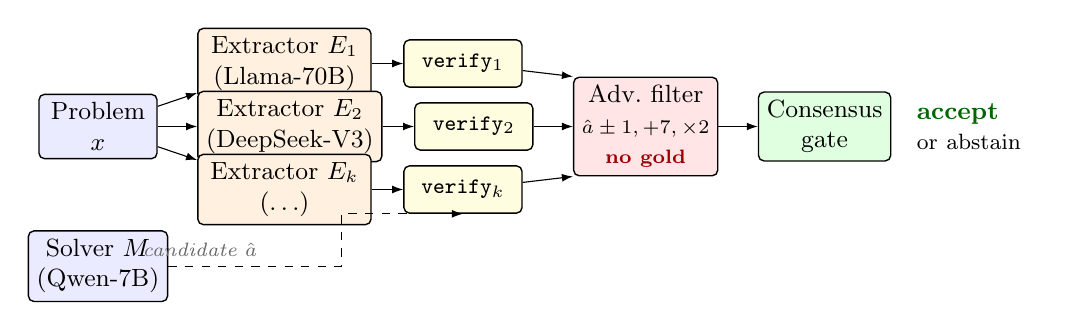
\begin{tikzpicture}[
  node distance=3mm and 4mm,
  every node/.style={font=\small},
  box/.style={draw, rounded corners=2pt, inner sep=3pt, minimum height=6mm,
              align=center, line width=0.5pt},
  prob/.style={box, fill=blue!8, minimum width=15mm},
  ext/.style={box, fill=orange!12, minimum width=22mm},
  ver/.style={box, fill=yellow!12, minimum width=15mm, font=\ttfamily\footnotesize},
  filt/.style={box, fill=red!10, minimum width=16mm},
  cons/.style={box, fill=green!12, minimum width=14mm},
  sol/.style={box, fill=blue!8, minimum width=15mm},
  arr/.style={-{Latex[length=1.4mm,width=1mm]}, line width=0.4pt},
  note/.style={font=\scriptsize\itshape, color=black!60},
]
  \node[prob] (p) {Problem\\$x$};
  \node[ext, right=5mm of p, yshift=8mm]  (e1) {Extractor $E_1$\\(Llama-70B)};
  \node[ext, right=5mm of p]              (e2) {Extractor $E_2$\\(DeepSeek-V3)};
  \node[ext, right=5mm of p, yshift=-8mm] (ek) {Extractor $E_k$\\ ($\ldots$)};
  \node[ver, right=4mm of e1] (v1) {verify$_1$};
  \node[ver, right=4mm of e2] (v2) {verify$_2$};
  \node[ver, right=4mm of ek] (vk) {verify$_k$};
  \node[filt, right=5mm of v2] (f) {Adv.\ filter\\{\scriptsize $\hat a \pm 1, +7, \times 2$}\\{\scriptsize\textcolor{red!60!black}{\textbf{no gold}}}};
  \node[cons, right=5mm of f] (c) {Consensus\\gate};
  \node[sol, below=9mm of p] (s) {Solver $M$\\(Qwen-7B)};
  \node[right=6mm of c] (out) {};

  \draw[arr] (p) -- (e1);
  \draw[arr] (p) -- (e2);
  \draw[arr] (p) -- (ek);
  \draw[arr] (e1) -- (v1);
  \draw[arr] (e2) -- (v2);
  \draw[arr] (ek) -- (vk);
  \draw[arr] (v1) -- (f.north west);
  \draw[arr] (v2) -- (f);
  \draw[arr] (vk) -- (f.south west);
  \draw[arr] (f) -- (c);
  \draw[arr, dashed] (s.east) -- ++(8mm, 0) node[note, midway, above] {candidate $\hat a$} -- ++(14mm, 0) |- (vk.south);
  \node[right=2mm of c, text width=14mm, align=left]
        {\small\textcolor{green!40!black}{\textbf{accept}}\\{\footnotesize or abstain}};
\end{tikzpicture}
\caption{X-SGRV pipeline. Each cross-family extractor reads only the problem $x$ and emits a Python/SymPy \texttt{verify} function. The deployment-time adversarial filter probes the verifier against perturbations of the candidate (never the gold). The consensus gate accepts only when every extractor produces a working verifier and every verifier accepts $\hat a$.}
\label{fig:pipeline}
\end{figure*}

\textbf{Setup.} Given a math problem $x$ and a candidate answer $\hat a$ from a solver LLM, we decide whether to accept $\hat a$ or abstain. We want a signal with high top-tier precision that does not collapse on contamination-clean data.

\textbf{Extraction.} A cross-family LLM $E$ reads only $x$ and emits a Python function \texttt{verify(answer) -> bool} using \texttt{sympy}, \texttt{math}, \texttt{itertools}, and \texttt{fractions}. If the problem cannot be checked by bounded enumeration or direct constraint substitution, $E$ returns the token \texttt{UNVERIFIABLE} and the pipeline abstains. The extractor never sees the solver's solution.

\textbf{Deployment-time adversarial filter.} We probe the verifier against $\{\hat a{-}1, \hat a{+}1, \hat a{+}7, 2\hat a, 42\}$. The probe set never references the gold answer and is safe at deployment. Any verifier that accepts a nearby wrong value is marked broken and the pipeline abstains. The probe set was fixed on a 30-problem held-out dev split disjoint from evaluation.

\textbf{Cross-extractor consensus.} Two or more independent cross-family extractors run in parallel. The pipeline returns a top-tier accept only when every extractor produces a working verifier and every verifier accepts $\hat a$.

\textbf{Verifier example.} Listing~\ref{lst:verifier} shows a representative verifier emitted by Llama-3.3-70B for a MATH-500 linear-equation problem. The extractor re-derives the constraint from the problem statement; the gold answer satisfies it; the adversarial filter rejects all perturbations.

\begin{figure}[t]
\begin{lstlisting}[style=xsgrv,caption={Representative X-SGRV verifier emitted by Llama-3.3-70B for a MATH-500 linear-equation problem.},label={lst:verifier}]
def verify(answer):
    try:
        x = int(str(answer).strip())
        return 5*x - 3*x + 4*(1 - 4*x) == 32
    except Exception:
        return False
\end{lstlisting}
\end{figure}

%==============================================================================
\section{Experimental Setup}
%==============================================================================

\textbf{Benchmarks.} MATH-500~\citep{hendrycks2021math, lightman2024prm} full ($n{=}498$, modulo two solver-timeout drops); MATH-500 stratified ($n{=}175$); AIME 2025 ($n{=}30$, post-Qwen cutoff); CleanMath ($n{=}125$: HMMT Feb 2025, BRUMO 2025, SMT 2025, APEX 2025 via \citet{matharena2025}); Omni-MATH hard-100~\citep{omnimath2024}; PutnamBench~\citep{amitayusht2024putnambench} 100-problem subset.

\textbf{Solvers.} Primary solver: Qwen2.5-7B-Instruct-Turbo~\citep{yang2024qwen25math}. Solver rotation: DeepSeek-V3, DeepSeek-R1, DeepSeek-V3.1, gpt-oss-120b.

\textbf{Extractors.} Six independent cross-family extractors spanning every major frontier lab: Meta (Llama-3.3-70B), DeepSeek (V3), OpenAI open-weights (gpt-oss-120b), Anthropic (Claude Sonnet 4.6), Alibaba (Qwen3-Coder-480B), and OpenAI (GPT-5-mini).

\textbf{Baselines.} Self-consistency $k{=}4$~\citep{wang2023selfconsistency}; verbalized confidence~\citep{xiong2024llmuncertainty}; p(True)~\citep{kadavath2022}; semantic entropy with SymPy equivalence and with NLI-DeBERTa clustering~\citep{kuhn2023semantic, farquhar2024nature}; Qwen2.5-Math-PRM-7B~\citep{qwenprm2025}; Skywork-o1-Open-PRM-Qwen-2.5-7B~\citep{skyworkprm2024}.

\textbf{Pre-registration.} Before the $n{=}498$ MATH-500 scale-up ran, we committed three narrative branches by consensus precision (A: $\geq 99\%$, B: 95--99\%, C: $<95\%$) to the project repository. The pre-registration also commits to reporting all PRM aggregations (min, mean, last, product) in the same table to prevent post-hoc selection.

\textbf{Generation settings.} Solver sampling uses temperature $T{=}0.7$ with 10 samples per problem for entropy baselines, and greedy ($T{=}0$) for the plurality candidate. Extractor calls use $T{=}0.2$ with \texttt{max\_tokens=2048}. Verifier scripts run in a subprocess sandbox with a 10-second wall-clock timeout.

%==============================================================================
\section{Results}
%==============================================================================

\begin{figure*}[t]
\centering
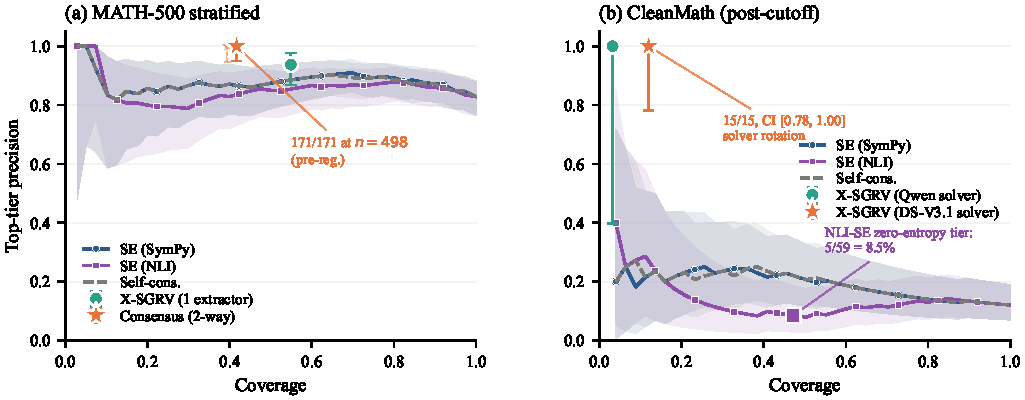
\includegraphics[width=0.92\linewidth]{figures/fig_workshop_precision_coverage.pdf}
\caption{Top-tier precision as a function of coverage on MATH-500 stratified (a) and on the post-cutoff CleanMath combo (b). Continuous baselines sweep their threshold; X-SGRV appears as a point (binary verdict) with Clopper-Pearson 95\% CI. On CleanMath, NLI-SE's zero-entropy tier is dominated by confidently-wrong answers (5/59 = 8.5\% precision); X-SGRV is the only method with a non-empty high-precision tier.}
\label{fig:pc}
\end{figure*}

\textbf{R1. Pre-registered consensus result.} On the full MATH-500 ($n{=}498$), Llama-3.3-70B~$\cap$~DeepSeek-V3 consensus yields $171/171 = 1.000$ [0.979, 1.000] at 34.3\% coverage --- the Branch A outcome. Single-extractor precision: Llama 230/243 = 0.947 [0.910, 0.971] at 48.8\% coverage; DeepSeek 199/207 = 0.961 [0.925, 0.983] at 41.6\% coverage. The Clopper-Pearson 95\% lower bound on consensus precision is 97.9\% with zero observed false positives.

\textbf{R2. Consensus is lab-agnostic.} On the stratified $n{=}175$ subsample, adding four more extractors (gpt-oss-120b, Claude Sonnet 4.6, Qwen3-Coder-480B, GPT-5-mini) preserves perfect precision as the tier shrinks: 2-way 73/73 = 1.000 at 41.7\% coverage, 4-way 72/72 at 41.1\%, 5-way 69/69 at 39.4\%, 6-way 67/67 at 38.3\%. Under an independent-extractor model, the consensus false-positive rate is bounded above by $p^k$ where $p$ is the per-extractor false-positive rate; the empirical $0/171$ on MATH-500 is consistent with this bound.

\textbf{R3. Contamination-clean behavior: coverage collapses, precision holds.} On AIME 2025, the deployment-time filter raises Llama's precision from 1/2 = 0.500 to 1/1 = 1.000 at 3.3\% coverage by catching one broken verifier. On CleanMath, Llama with the original Qwen solver reaches 4/4 = 1.000 [0.40, 1.00] at 3.2\% coverage. A solver rotation to DeepSeek-V3 tightens this to 9/9 = 1.000 [0.66, 1.00] and to DeepSeek-V3.1 gives 15/15 = 1.000 [0.78, 1.00], without changing the extractor scripts (Figure~\ref{fig:pc}b). The rotation rules out the alternative that selective-prediction behavior is an artifact of the 7B solver: a stronger solver produces more correct candidates for the same verifier scripts to accept, and the X-SGRV tier grows proportionally while precision holds.

\textbf{R4. Baselines collapse on contamination-clean benchmarks.} On AIME 2025, NLI-clustering semantic entropy's zero-entropy tier contains 16/30 problems with only 1 correct (6.2\% precision, AUROC 0.420). On CleanMath, NLI-SE gives 5/59 = 8.5\% precision at 47\% coverage (Figure~\ref{fig:pc}b). SymPy-clustering SE achieves AUROC 0.735 on CleanMath but the zero-entropy tier contains only 6/125 problems with 1 correct. p(True) AUROC is 0.463 on AIME 2025 and 0.474 on CleanMath --- both worse than random. Template SGRV, ExeVer, and SC-4 all produce empty top tiers on AIME 2025. Across five baselines spanning entropy-, agreement-, and template-based families, none retains a non-empty high-precision tier under contamination-clean shift, leaving X-SGRV as the only signal in our comparison set with measurable selective-prediction value on these benchmarks.

\textbf{R5. X-SGRV is competitive with the best open PRMs.} Table~\ref{tab:prm} reports the matched-coverage comparison. On MATH-500 at 54.9\%, X-SGRV, Qwen-PRM (min-step), and Skywork-PRM (min-step) are tied within CI at 0.93--0.94. On CleanMath at 3.2\%, Qwen-PRM's best aggregation reaches only 0.500 while Skywork-PRM (mean) and X-SGRV both reach 1.000. The Qwen-PRM degradation is consistent with its training distribution being concentrated on MATH-family problems, while Skywork-PRM's broader training distribution preserves out-of-distribution generalization. X-SGRV reaches matched precision through spec-grounded SymPy verification, with no training signal.

\begin{table}[t]
\centering
\caption{X-SGRV vs.\ open PRMs at matched coverage (X-SGRV's top-tier coverage on each benchmark; Clopper-Pearson 95\% CIs). MATH is the stratified $n{=}175$ subsample.}
\label{tab:prm}
\footnotesize
\setlength{\tabcolsep}{3pt}
\begin{tabular}{@{}llrl@{}}
\toprule
Method & Bench & Cov. & Precision (95\% CI) \\
\midrule
X-SGRV (Llama-70B)   & MATH  & 54.9\% & \textbf{0.938} [0.87, 0.98] \\
Qwen-PRM-7B, min     & MATH  & 54.9\% & 0.927 [0.86, 0.97] \\
Skywork-PRM-7B, min  & MATH  & 54.9\% & \textbf{0.938} [0.87, 0.98] \\
\midrule
X-SGRV (Llama-70B)   & AIME  &  6.7\% & 0.500 [0.01, 0.99] \\
Qwen-PRM-7B, min     & AIME  &  6.7\% & 0.500 [0.01, 0.99] \\
Skywork-PRM-7B, mean & AIME  &  6.7\% & 0.500 [0.01, 0.99] \\
\midrule
X-SGRV (Llama-70B)   & Clean &  3.2\% & \textbf{1.000} [0.40, 1.00] \\
Qwen-PRM-7B, best    & Clean &  3.2\% & 0.500 [0.07, 0.93] \\
Skywork-PRM-7B, mean & Clean &  3.2\% & \textbf{1.000} [0.40, 1.00] \\
\bottomrule
\end{tabular}
\end{table}

\textbf{R6. Lean and SymPy are complementary.} On 90 problems (60 MATH + 30 AIME), frontier LLMs emit Lean 4 theorems that compile and type-check against Mathlib in a sandbox: Claude Sonnet 4.6 71/90 = 78.9\%, GPT-5-mini 57/75 = 76.0\%, DeepSeek-V3 28/81 = 34.6\%. The compile-check does not verify whether the theorem statement matches the problem, since an LLM can emit a trivially-true statement that type-checks. We therefore do not claim Lean is worse than SymPy. We position the two approaches as complementary: SymPy compiles on every working verifier by construction and executes in the same Python sandbox as the solver, which preserves the gold-free adversarial filter; Lean offers stronger soundness guarantees on the problems where compilation succeeds and the theorem matches.

%==============================================================================
\section{Limitations}
%==============================================================================

\textbf{First, X-SGRV has an operational ceiling on proof-style problems.} On Omni-MATH hard-100~\citep{omnimath2024} (difficulty 9.0--9.5), zero verifiers meet the working criterion and the single tier acceptance is a false positive. On 100 PutnamBench problems~\citep{amitayusht2024putnambench}, Claude Sonnet 4.6 correctly returns \texttt{UNVERIFIABLE} on 51\% by design and produces a verifier that accepts the gold on 19\%; GPT-5-mini refuses 35\% and accepts 8\%. The refusal rates are evidence that extractors detect their own scope limit, but the method is not a substitute for a proof assistant on proof-heavy problems.

\textbf{Second, the CleanMath confidence interval is wide under the primary solver.} The 4/4 point estimate with the Qwen solver has a Clopper-Pearson lower bound of 40\%; solver rotation tightens this to 66--78\% but does not close it. Coverage remains single-digit on contamination-clean benchmarks. We report this as a feature of correct abstention rather than a robustness gap, but it means X-SGRV is not a coverage-maximizing replacement for continuous-score selective prediction.

\textbf{Third, extractor size and family are entangled.} Our same-family ablation (Qwen2.5-7B as the extractor) drops the non-abstain rate to 12\% on MATH and 7\% on AIME, but this confounds family with scale (7B vs.\ 70B+). The Llama-70B vs.\ DeepSeek-V3 cross-family comparison at matched scale is the cleanest available test of the family axis. Distilling the 70B extractor into a smaller model is open work.

%==============================================================================
\section{Related Work}
%==============================================================================

\textbf{Self-verification and code-based checking.} \citet{exever} introduced same-model Python/SymPy verification, our baseline. \citet{symcode2024, mathvf2025} translate solutions to formal representations for deterministic checking. \citet{dtv2024} used Isabelle autoformalization for specification-grounded verification, the closest prior to our independence framing. \citet{deepseekmathv2} train self-verifiable reasoning within a single family, preserving the solver/verifier correlation that X-SGRV is designed to break.

\textbf{Process reward models.} \citet{lightman2024prm} introduced the PRM800K dataset; \citet{mathshepherd2024} generated step labels via Monte Carlo estimation; \citet{qwenprm2025, skyworkprm2024} are the open PRM state of the art we benchmark against. \citet{rstarmath2025, prime2025, acemath2024} provide additional training paradigms; we leave broader PRM sweeps as future work.

\textbf{Selective prediction and uncertainty.} \citet{xiong2024llmuncertainty} document overconfidence in verbalized estimates; \citet{kadavath2022} introduced p(True); \citet{kuhn2023semantic, farquhar2024nature} introduced semantic entropy. We benchmark against all of these.

\textbf{Correlated errors.} \citet{huang2024selfcorrect, tyen2024llm, stechly2024selfverify} establish that intrinsic self-correction degrades reasoning. \citet{kim2025correlated} show correlated errors grow with model scale.

\textbf{Contamination.} \citet{wu2025contam} demonstrate the MATH-500 reproduction phenomenon that motivates our contamination-clean evaluation. \citet{olympiadbench2024, omnimath2024, matharena2025, mathperturb2025} provide contamination-cleaner benchmarks.

%==============================================================================
\section{Conclusion}
%==============================================================================

\textbf{Summary.} Same-model self-verification on MATH-500 has a 13.8\% false acceptance rate that scales monotonically with difficulty, and every standard agreement- or template-based selective-prediction signal we test collapses on contamination-clean benchmarks. X-SGRV uses a large cross-family LLM extractor to emit SymPy verifier scripts from the problem statement, combined with a gold-free adversarial filter and cross-extractor consensus. The pre-registered MATH-500 $n{=}498$ consensus precision is $171/171 = 1.000$ [0.979, 1.000] at 34.3\% coverage. On AIME 2025 and CleanMath, coverage drops to 3--12\% while precision remains at or near perfect; solver rotation tightens the CI without changing the extractor.

\textbf{Limitations.} First, X-SGRV is scoped to find-style problems and cannot handle proof-heavy olympiad questions, where the extractor correctly refuses on more than half of PutnamBench. Second, contamination-clean confidence intervals are wide under weak solvers and tighten only with solver rotation. Third, the same-family ablation entangles extractor scale with extractor family, leaving the cleanest test of the family axis to the Llama-70B vs.\ DeepSeek-V3 cross-family comparison.

\textbf{Implications for future research.} A hybrid SymPy-plus-Lean pipeline routed by the extractor's \texttt{UNVERIFIABLE} signal is a direct next step, supported by Claude's 78.9\% Mathlib compile rate. Distilling the 70B extractor into a smaller model would broaden deployment. Formalizing the convergence-to-one behavior of cross-extractor consensus would replace the current empirical bound with a guarantee. Cross-method, cross-benchmark contamination-collapse measurements should become standard practice for new selective-prediction proposals.

\textbf{Field actions.} MATH-500 numbers for Qwen-family solvers should be reported as upper bounds and AIME-2025-and-later benchmarks as the realistic operating point. Open process reward models should be evaluated on contamination-clean data before being published as state of the art; the Qwen-PRM degradation from 0.927 to 0.500 on CleanMath is invisible if only MATH-500 is reported. Selective-prediction papers should pre-register their headline numbers on full benchmarks, with narrative branches committed in advance.

\textbf{Reproducibility.} All benchmarks are public; all extractors are public API or open-weights models; code, prompts, the held-out probe set, and raw JSON results are released with the submission.

\bibliographystyle{icml2025}
\bibliography{references}

\end{document}
